
\chapter{Projections of the main fit to data}
\label{app:main_fit}

\begin{figure}[tp]
    \centering
    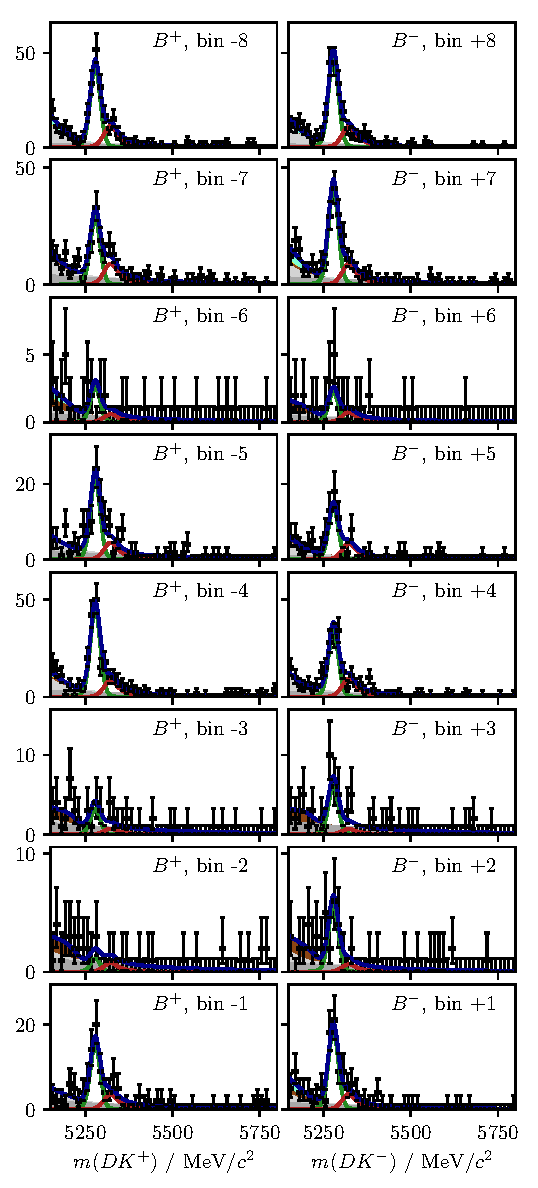
\includegraphics[height=6in]{figures/analysis/bin_by_bin/pretty_fit_bins_dk_LL_1.pdf}
    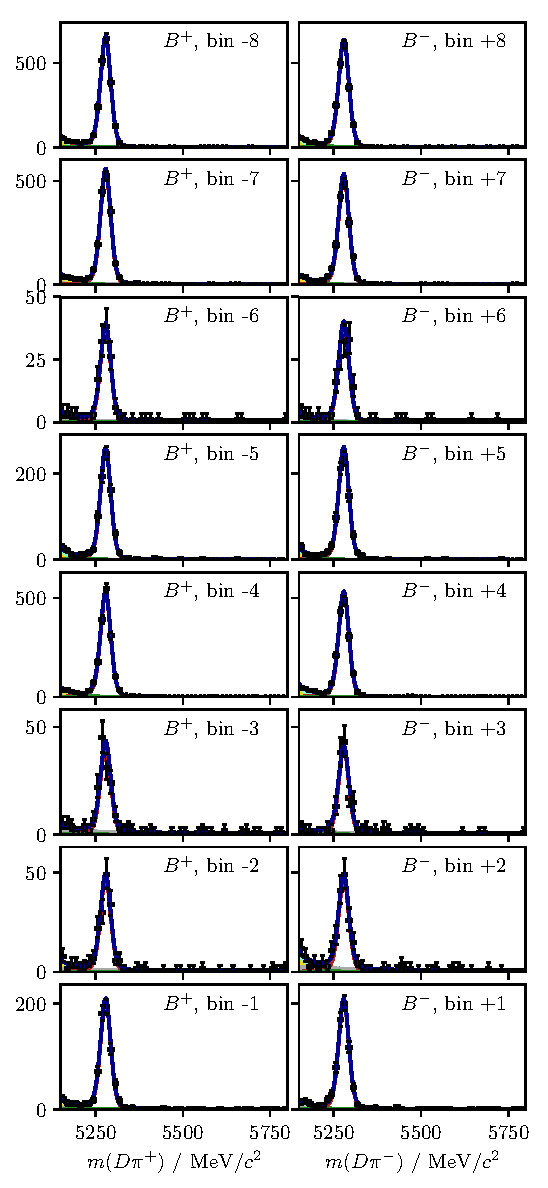
\includegraphics[height=6in]{figures/analysis/bin_by_bin/pretty_fit_bins_dpi_LL_1.pdf}
    \caption{Projections of the main fit to data described in Section~\ref{sec:measurement_of_the_cp_violation_observables}. The two columns on the left show \BtoDK candidates, split by charge, while the two columns on the right show \BtoDpi candidates. These projections are for the \DtoKspp mode where the \KS meson is in the LL category.}
\end{figure}

\begin{figure}[tp]
    \centering
    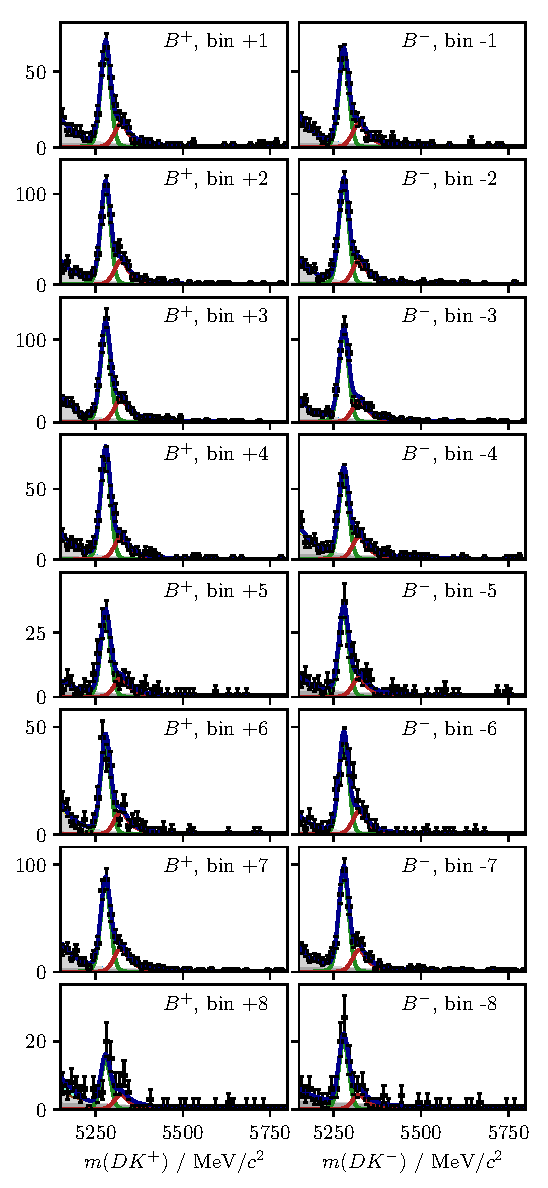
\includegraphics[height=6in]{figures/analysis/bin_by_bin/pretty_fit_bins_dk_LL_2.pdf}
    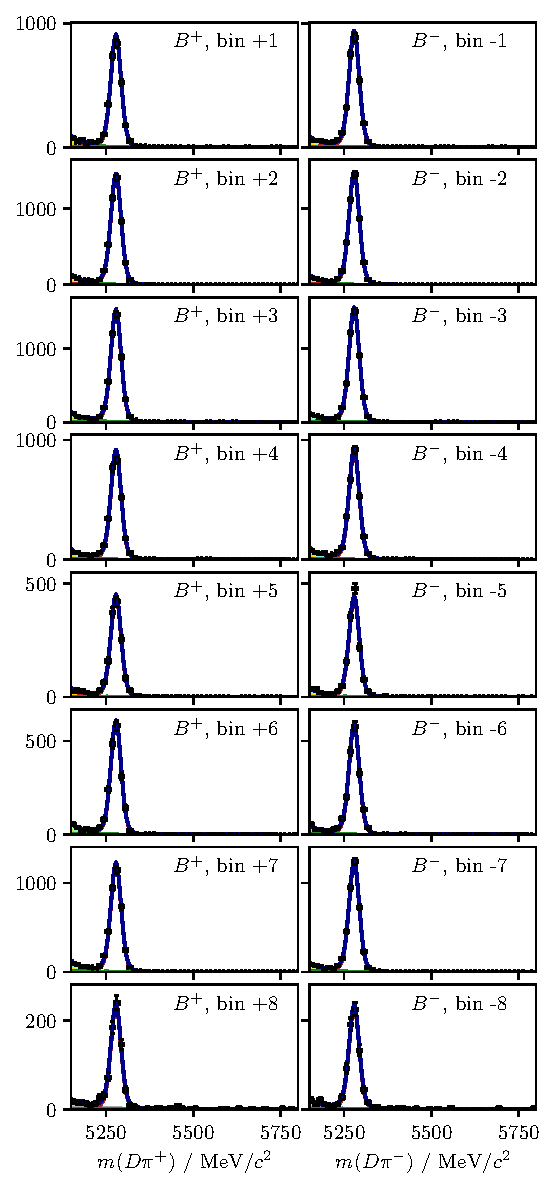
\includegraphics[height=6in]{figures/analysis/bin_by_bin/pretty_fit_bins_dpi_LL_2.pdf}
    \caption{Projections of the main fit to data described in Section~\ref{sec:measurement_of_the_cp_violation_observables}. The two columns on the left show \BtoDK candidates, split by charge, while the two columns on the right show \BtoDpi candidates. These projections are for the \DtoKspp mode where the \KS meson is in the LL category.}
\end{figure}

\begin{figure}[tp]
    \centering
    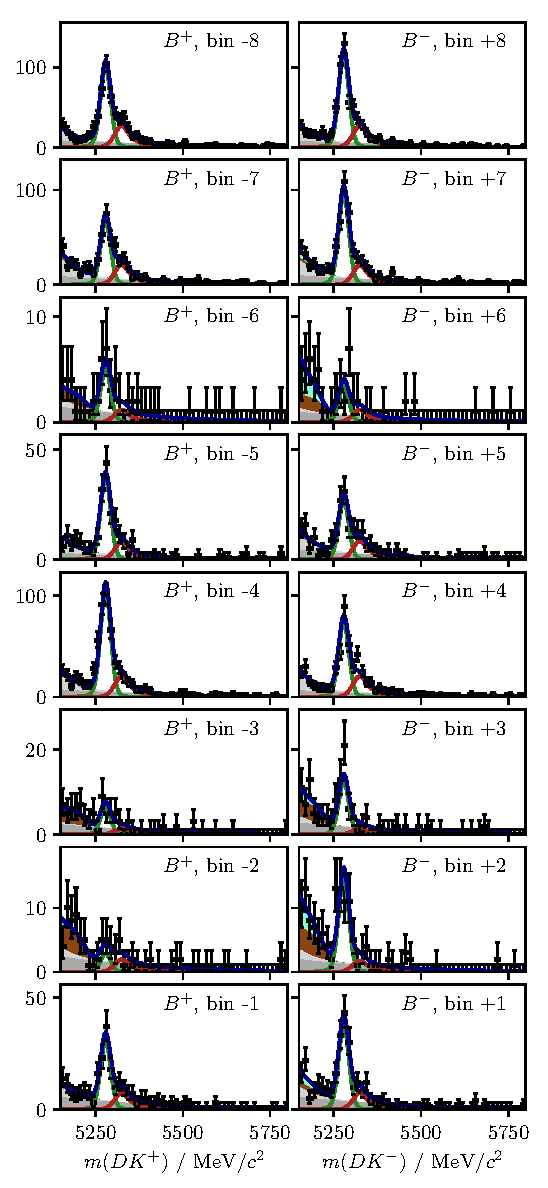
\includegraphics[height=6in]{figures/analysis/bin_by_bin/pretty_fit_bins_dk_DD_1.pdf}
    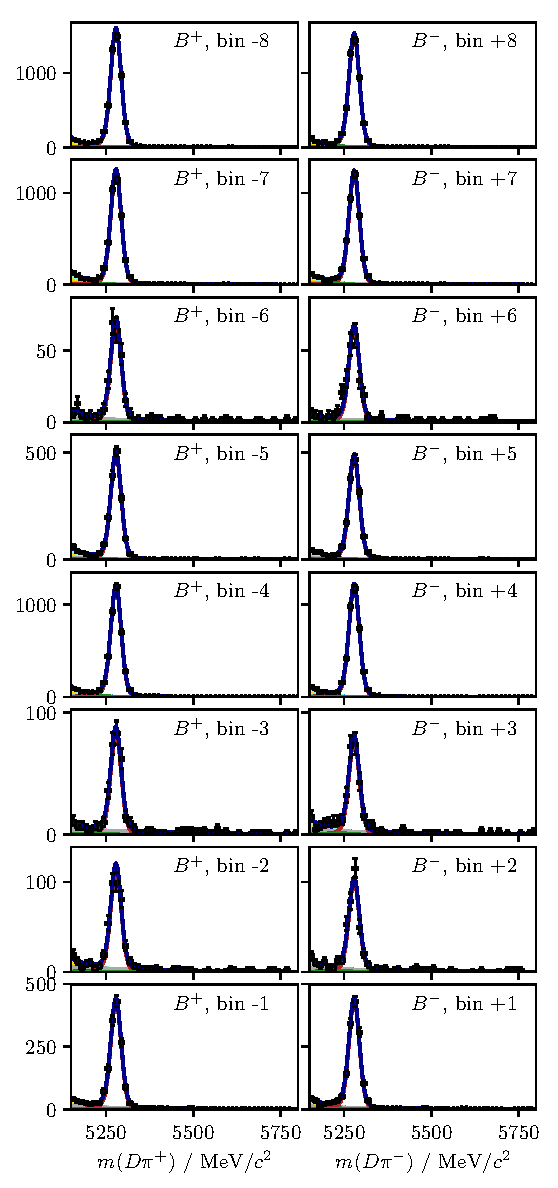
\includegraphics[height=6in]{figures/analysis/bin_by_bin/pretty_fit_bins_dpi_DD_1.pdf}
    \caption{Projections of the main fit to data described in Section~\ref{sec:measurement_of_the_cp_violation_observables}. The two columns on the left show \BtoDK candidates, split by charge, while the two columns on the right show \BtoDpi candidates. These projections are for the \DtoKspp mode where the \KS meson is in the DD category.}
\end{figure}

\begin{figure}[tp]
    \centering
    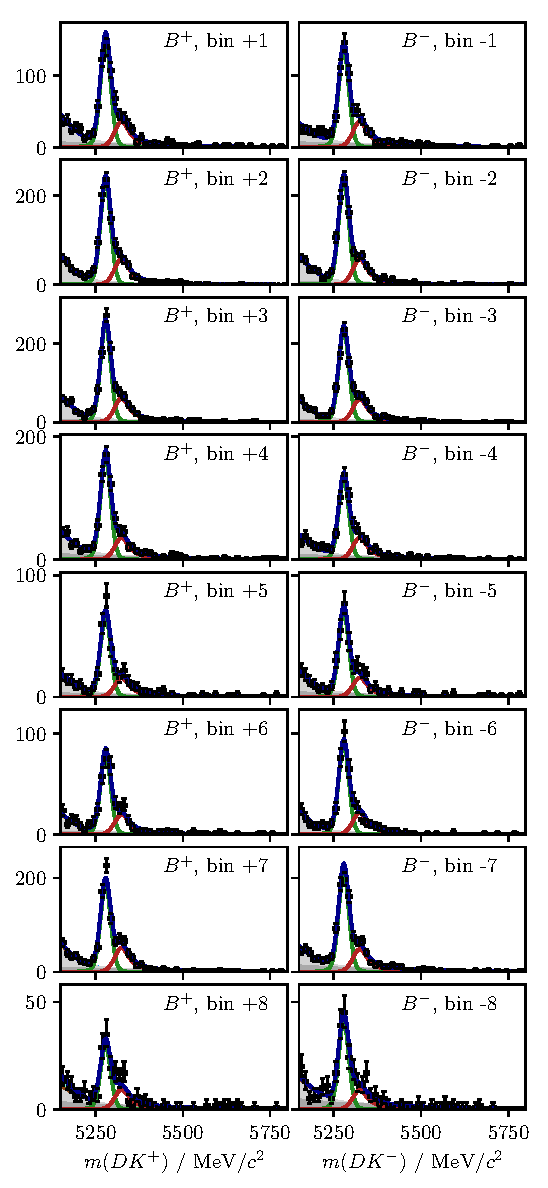
\includegraphics[height=6in]{figures/analysis/bin_by_bin/pretty_fit_bins_dk_DD_2.pdf}
    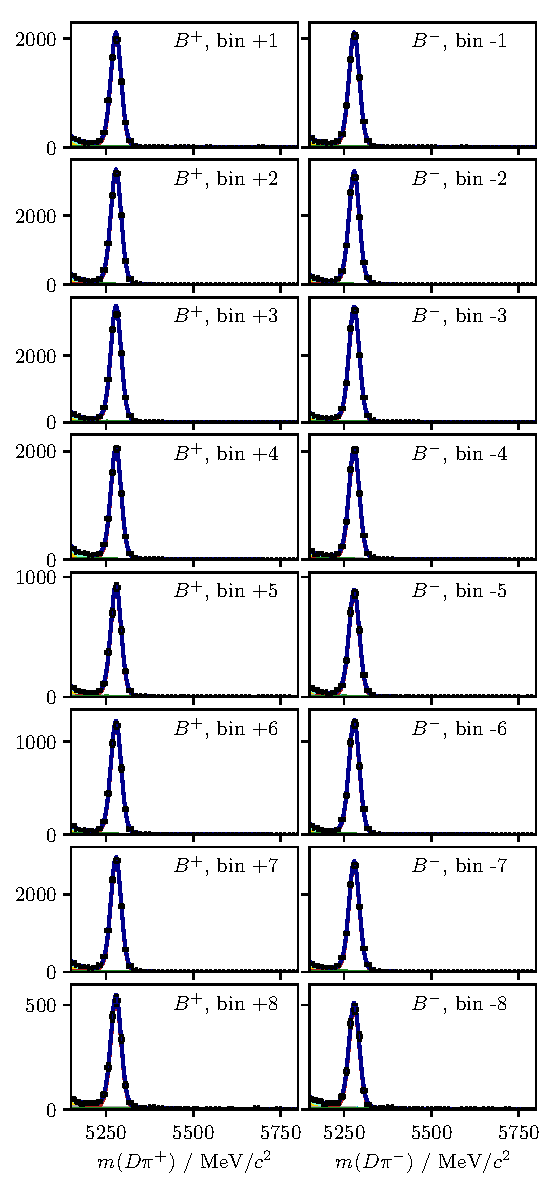
\includegraphics[height=6in]{figures/analysis/bin_by_bin/pretty_fit_bins_dpi_DD_2.pdf}
    \caption{Projections of the main fit to data described in Section~\ref{sec:measurement_of_the_cp_violation_observables}. The two columns on the left show \BtoDK candidates, split by charge, while the two columns on the right show \BtoDpi candidates. These projections are for the \DtoKspp mode where the \KS meson is in the DD category.}
\end{figure}

\begin{figure}[tp]
    \centering
    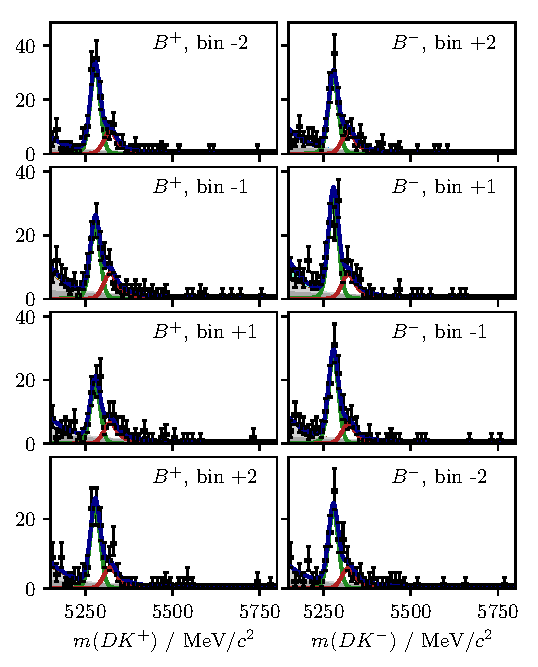
\includegraphics[height=3.5in]{figures/analysis/bin_by_bin/pretty_fit_bins_dk_LL_1_d2kskk.pdf}
    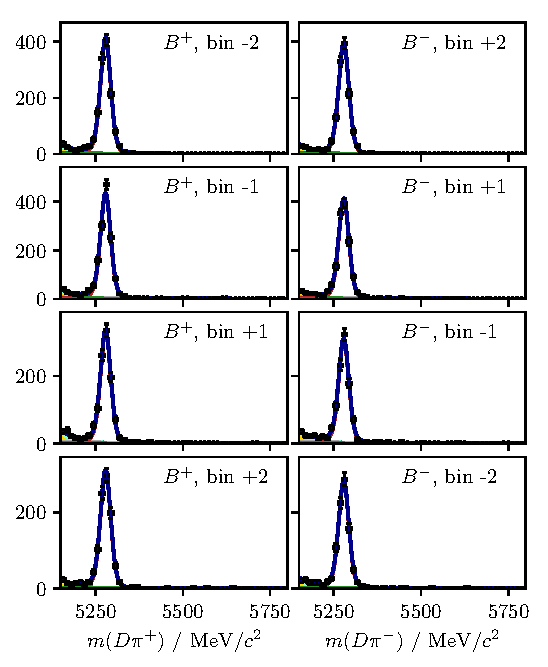
\includegraphics[height=3.5in]{figures/analysis/bin_by_bin/pretty_fit_bins_dpi_LL_1_d2kskk.pdf}
    \caption{Projections of the main fit to data described in Section~\ref{sec:measurement_of_the_cp_violation_observables}. The two columns on the left show \BtoDK candidates, split by charge, while the two columns on the right show \BtoDpi candidates. These projections are for the \DtoKskk mode where the \KS meson is in the LL category.}
\end{figure}

\begin{figure}[tp]
    \centering
    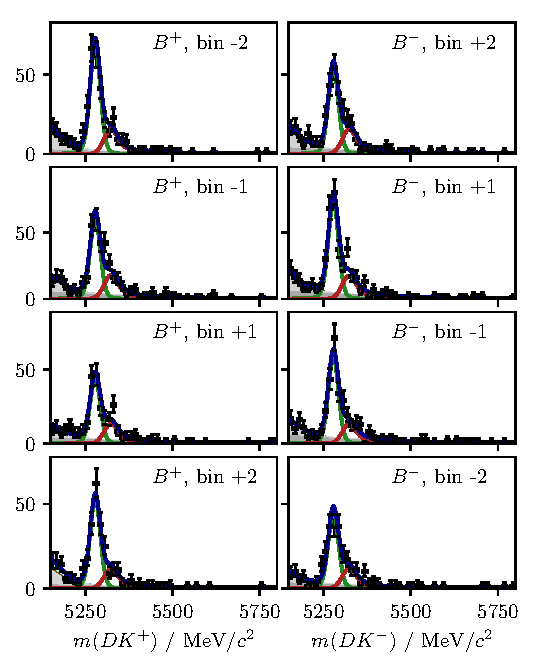
\includegraphics[height=3.5in]{figures/analysis/bin_by_bin/pretty_fit_bins_dk_DD_1_d2kskk.pdf}
    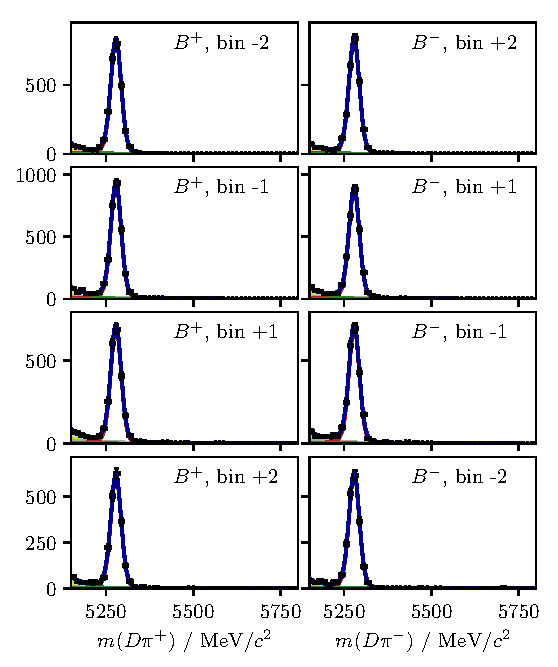
\includegraphics[height=3.5in]{figures/analysis/bin_by_bin/pretty_fit_bins_dpi_DD_1_d2kskk.pdf}
    \caption{Projections of the main fit to data described in Section~\ref{sec:measurement_of_the_cp_violation_observables}. The two columns on the left show \BtoDK candidates, split by charge, while the two columns on the right show \BtoDpi candidates. These projections are for the \DtoKskk mode where the \KS meson is in the DD category.}
\end{figure}